\subsection{Modelos de Ehrenfest}
% http://www.math.uah.edu/stat/markov/Ehrenfest.html
% https://www.dartmouth.edu/~chance/teaching_aids/books_articles/probability_book/Chapter11.pdf
% http://www.math.uiuc.edu/~rsong/488f02/ch8.pdf

\begin{questions}
\question{
Paul Ehrenfest propôs um modelo simples para a troca de calor ou moléculas entre
dois corpos isolados. Neste modelo da cadeia de Ehrenfest iremos considerar a troca de
moléculas de gás entre dois compartimentos, rotulados por 0 e 1,
conforme apresentado na Figura \ref{fig:ehrenfes}.

\begin{figure}[h]
    \centering
    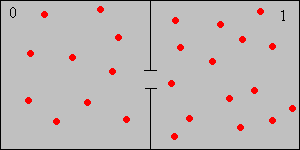
\includegraphics[width=0.3\textwidth]{../images/ehrenfest.png}
    \caption{Modelo de Ehrenfest.}
    \label{fig:ehrenfes}
\end{figure}

O número total de partículas no sistema é $m$.
O estado do sistema em qualquer instante $n$ pode ser descrito pelo
número de partículas no compartimento 1. Iremos então denotar por $X_n$ este número.
Temos um processo estocástico gerando uma sequência de variáveis aleatórias $X_{1:n}$
que assumem valor em $\{0,1,\ldots,m\}$.

Uma das $m$ partículas no sistema é selecionada aleatoriamente, a cada instante,
e esta partícula troca de compartimento. Supondo que, no instante $n$,
o compartimento 1 possua $i$ bolas, o modelo de Ehrenfest nos
fornece as seguintes probabilidades
\begin{eqnarray}
\Pr(X_{n+1} = i+1 | X_n = i) &=& \frac{m - i}{m} , \nonumber  \\
\Pr(X_{n+1} = i-1 | X_n = i) &=& \frac{i}{m} .
\end{eqnarray}
Podemos observar que neste processo, a probabilidade condicional é a mesma, se
condicionarmos a todo histórico do processo até o instante $n$, ou seja,
\begin{eqnarray}
\Pr(X_{n+1} = i+1 | X_0 = i_0, X_1 = i_1, \ldots, X_{n-1} = i_{n-1}, X_n = i) &=& \Pr(X_{n+1} = i+1 | X_n = i) , \nonumber \\
\Pr(X_{n+1} = i-1 | X_0 = i_0, X_1 = i_1, \ldots, X_{n-1} = i_{n-1}, X_n = i) &=& \Pr(X_{n+1} = i-1 | X_n = i) .
\end{eqnarray}
Esta propriedade é a propriedade de Markov, que diz que futuro e passado são independentes, dado o presente.
Podemos verificar também que a distribuição condicional não depende de $n$, desta forma, temos um processo
estocástico homogêneo. A cadeia de Markov poderá então ser descrita por uma matriz de transição fixa $P = [p_{ij}]_{ij}$.

Vamos considerar o caso em que $m=4$ e faça o que se pede:
\begin{parts}
\part Faça o grafo da cadeia de Markov.
\part Encontre a matriz de transição.
\part Calcule a distribuição de estado estacionário. 
\part Calcule a taxa de entropia do processo.
\end{parts}
}

\begin{solution}
\begin{parts}
\part
\begin{center}
\begin{tikzpicture}[->, >=stealth', auto, semithick, node distance=3cm]
\tikzstyle{every state}=[fill=white,draw=black,thick,text=black,scale=1]
\node[state]    (0)               {$0$};
\node[state]    (1)[right of=0]   {$1$};
\node[state]    (2)[right of=1]   {$2$};
\node[state]    (3)[right of=2]   {$3$};
\node[state]    (4)[right of=3]   {$4$};
\path
(0) edge[bend left,above]   node{$1$}    (1)
(1) edge[bend left,below]   node{$1/4$}  (0)
(1) edge[bend left,above]   node{$3/4$}  (2)
(2) edge[bend left,below]   node{$1/2$}  (1)
(2) edge[bend left,above]   node{$1/2$}  (3)
(3) edge[bend left,below]   node{$3/4$}  (2)
(3) edge[bend left,above]   node{$1/4$}  (4)
(4) edge[bend left,below]   node{$1$}    (3) ;
% edge[loop left]     node{$p^2$}         (1) ;
\end{tikzpicture}
\end{center}


\part
Para $m=4$, a matriz de transição ser
\begin{equation}
\mathbf{P} = 
\begin{blockarray}{cccccc}
0 & 1 & 2 & 3 & 4 \\
\begin{block}{(ccccc)c}
  0   & 1   & 0   & 0   & 0   & 0 \\
  1/4 & 0   & 3/4 & 0   & 0   & 1 \\
  0   & 1/2 & 0   & 1/2 & 0   & 2 \\
  0   & 0   & 3/4 & 0   & 1/4 & 3 \\
  0   & 0   & 0   & 1   & 0   & 4 \\
\end{block}
\end{blockarray}
\end{equation}

A distribuição de estado estacionário é tal que $\mathbf{\mu}^T P = \mathbf{\mu}^T$, com $\sum_i \mu_i = 1$.

\begin{eqnarray}
\mathbf{\mu}^T P &=& \mathbf{\mu}^T \nonumber \\
\mathbf{\mu}^T (P-I) &=& 0 \nonumber \\
\mathbf{\mu}^T Q &=& 0 
\end{eqnarray}

Teremos aqui
\begin{equation}
Q = \begin{pmatrix} 
-1  &  1  & 0   & 0   & 0   \\
1/4 & -1  & 3/4 & 0   & 0   \\
0   & 1/2 & -1  & 1/2 & 0   \\
0   & 0   & 3/4 & -1  & 1/4 \\
0   & 0   & 0   & 1   & -1
\end{pmatrix} .
\end{equation}


Note que, no sistema de equações acima,
as colunas de $P$, e consequentemente as colunas de $Q$, são redundantes,
de forma que uma dada coluna qualquer pode ser obtida através das demais
pois sabemos que cada linha de $P$ deve somar um e, da mesma forma,
cada linha de $Q$ deve somar zero. Podemos assim, sem prejuízo,
substituir uma das colunas de $Q$ de forma a incorporar a condição $\sum_i \mu_i = 1$. Basta
para tanto substituir uma das colunas da matriz $Q$ por uma coluna com uns e substituir
um dos zeros no vetor de zeros, ao lado direito da equação, por um na posição respectiva.
Podemos, por exemplo, escolher a última coluna de $Q$ e assim teremos uma matriz
\begin{equation}
\tilde{Q} = \begin{pmatrix} 
-1  &  1  & 0   & 0   & 1 \\
1/4 & -1  & 3/4 & 0   & 1 \\
0   & 1/2 & -1  & 1/2 & 1 \\
0   & 0   & 3/4 & -1  & 1 \\
0   & 0   & 0   & 1   & 1
\end{pmatrix} ,
\end{equation}
e o novo sistema de equações será
\begin{equation}
\mathbf{\mu}^T \tilde{Q} = (0, 0, 0, 1) .
\label{eq-novo-sistema}
\end{equation}
Observe que qualquer coluna de $Q$ é determinada pelas demais colunas de $Q$, levando-se
em consideração que a soma em cada linha de $Q$ deve ser igual a $1$, já que uma linha de $Q$
representa a probabilidade de transição a um outro estado a partir do estado associado pela
linha de $Q$ em questão. Podemos então incorporar a condição $\sum_i \mu_i = 1$ substituindo
como proposto anteriormente, ou seja, substituindo uma coluna de $Q$ (por exemplo a $j$-ésima coluna)
por uma coluna de uns, obtendo assim a matriz $\tilde{Q}$.
Ao realizar a multiplicação de $\mathbf{\mu}^T$ pela $j$-ésima coluna de $\tilde{Q}$,
denotada por $\tilde{q}_{\ast,j}$, teremos
\begin{equation} 
\mathbf{\mu}^T \tilde{q}_{\ast,j} = \begin{bmatrix}\mu_1 & \ldots & \mu_m \end{bmatrix} 
        \begin{bmatrix} 1\\ \vdots \\ 1 \end{bmatrix} =  \sum_i \mu_i = 1 ,
\end{equation}
incorporando assim a condição de que $\mathbf{\mu}$ deve pertencer ao simplex probabilístico.

Para solucionar a Equação \ref{eq-novo-sistema}, poderemos pós multiplicar ambos os lados
pela matriz inversa de $\tilde{Q}$,
\begin{equation}
\mathbf{\mu}^T = (0, 0, 0, 1) \tilde{Q}^{-1} .
\end{equation}


\begin{lstlisting}[language=Octave]
P = [0 1 0 0 0; 1/4 0 3/4 0 0; 0 1/2 0 1/2 0; 0 0 3/4 0 1/4; 0 0 0 1 0];
Q = P - eye(size(P));
Q2 = Q;
Q2(:,5)=ones(5,1);
[0 0 0 0 1]*inv(Q2)
ans =
  0.062500   0.250000   0.375000   0.250000   0.062500
\end{lstlisting}

\begin{equation}
\mathbf{\mu}^T = \left( \frac{1}{16}, \frac{1}{4}, \frac{6}{16}, \frac{1}{4}, \frac{1}{16} \right)
\end{equation}


A taxa de entropia para um cadeia de Markov de primeira ordem
estacionária será dada da seguinte forma
  \begin{eqnarray}
  H(\mathcal{X}) &=& H'(\mathcal{X}) = \lim_{n \rightarrow \infty} H(X_n \mid X_{n-1}, \ldots, X_1) \nonumber \\
        &=& \lim_{n \rightarrow \infty} H(X_n \mid X_{n-1}) \nonumber \\
        && \text{dado que é Markov de 1a ordem} \nonumber \\
        &=& H(X_2 \mid X_1) \quad \text{(estacionário)} \nonumber \\
        &=& - \sum_{x_2, x_1} p(x_2, x_1) \log p(x_2 \mid x_1) = \sum_i \mu_i \left[ - \sum_j p_{ij} \log p_{ij} \right] \nonumber \\
        &=& \sum_i \mu_i H( \mathbf{p_i} )
  \end{eqnarray}
onde $\mu$ é a distribuição estacionária,
$p_{ij}$ a probabilidade de transição de $i$ para $j$ (elementos da matriz $P$)
e $\mathbf{p_i}$ a $i$-ésima linha da matriz $P$ (as probabilidades de transição à partir
do estado $i$).

Para o nosso exemplo, teremos
\begin{eqnarray}
  H(\mathcal{X}) &=& \mu_1 H(\mathbf{p_1}) + \mu_2 H(\mathbf{p_2}) + \mu_3 H(\mathbf{p_3}) +
        \mu_4 H(\mathbf{p_4}) + \mu_5 H(\mathbf{p_5}) \nonumber \\
        &=& \frac{1}{16} H(0,1,0,0,0) + \frac{1}{4} H(\frac{1}{4}, 0, \frac{3}{4}, 0, 0) + 
                \frac{6}{16} H(0, \frac{1}{2}, 0, \frac{1}{2}, 0) + 
                \frac{1}{4} H(0, 0, \frac{3}{4}, 0, \frac{1}{4}) \nonumber \\
	    && + \frac{1}{16} H(0, 0, 0, 1, 0) \nonumber \\
        &=& 0 + 2 \times \frac{1}{4} \left( \frac{1}{4} \log 4 + \frac{3}{4} \log \frac{4}{3} \right) +
                \frac{6}{16} + 0 \nonumber \\
        &=& \frac{1}{2} \left( \frac{1}{2} + \frac{3}{2} - \frac{3}{4} \log 3  \right) + \frac{6}{16} \nonumber \\
        &=& 1 - \frac{3}{8} \log 3 + \frac{6}{16} = \frac{11}{8} - \frac{3}{8} \log 3 = 0.78064
\end{eqnarray}


Note que tomando $P^n$, para $n$ grande suficiente, verificaremos que $P^n$ converge
para uma matriz onde apenas duas linhas são distintas:
\begin{equation}
\mathbf{\mu}_1^T = \left( \frac{1}{8}, 0, \frac{3}{4}, 0, \frac{1}{8} \right) \quad \text{ e } \quad 
\mathbf{\mu}_2^T = \left(0, \frac{1}{2}, 0, \frac{1}{2}, 0 \right) ,
\end{equation}
sendo que $P^n$ será da forma
\begin{equation}
P^n = \begin{bmatrix} \mathbf{\mu}_1^T \\ \mathbf{\mu}_2^T \\ \mathbf{\mu}_1^T \\ \mathbf{\mu}_2^T \\ \mathbf{\mu}_1^T \end{bmatrix}
\end{equation}
Observe que, neste caso, não haverá estado estacionário, mas a distribuição sobre os estados
ficará oscilando entre $\mathbf{\mu}_1^T$ e $\mathbf{\mu}_2^T$.

\begin{lstlisting}[language=Octave]
function y=plogp(p)
  y = zeros(size(p));
  id = find(p>0);
  y(id) = p(id).*log2(p(id));
endfunction;

function H=entropy(p)
   H = -sum(plogp(p));
endfunction;

function H=markovEntropyRate(P,mu)
  if nargin < 2,
     Q = P - eye(size(P));
     Q1 = Q;
     Q1(:,end)=ones(size(P,1),1); 
     if det(Q1) == 0, % singular
        mu = [zeros(1,size(P,2)-1), 1] * pinv(Q1);
     else
        mu = [zeros(1,size(P,2)-1), 1] * inv(Q1);
     endif;
  endif;

  H=0;
  for i=1:size(P,1),
      H += mu(i)*(- sum( plogp( P(i,:) ) ) );
  endfor;
endfunction

P = [0 1 0 0 0; 1/4 0 3/4 0 0; 0 1/2 0 1/2 0; 0 0 3/4 0 1/4; 0 0 0 1 0];
H = markovEntropyRate(P);
\end{lstlisting}

Obverve novamente as equações:
\begin{eqnarray}
\mathbf{\mu}^T P &=& \mathbf{\mu}^T \label{eq-muPmu} \nonumber \\
\mathbf{\mu}^T Q &=& 0 \label{eq-muQ0}
\end{eqnarray}
Podemos verificar pela Equação \ref{eq-muPmu} que $\mu$ deverá ser um autovetor
à esquerda de $P$, com autovalor associado $1$. De forma equivalente, através
da Equação \ref{eq-muQ0}, deveremos ter que $\mu$ está no espaço nulo à esquerda de $Q$.
Tomando a transposta da Equações \ref{eq-muPmu}
\begin{eqnarray}
( \mathbf{\mu}^T P )^T &=& ( \mathbf{\mu}^T )^T \nonumber \\
P^T \mathbf{\mu} &=& \mathbf{\mu} \label{eq-muPmuT}  ,
\end{eqnarray}
e da Equação \ref{eq-muQ0} teremos
\begin{eqnarray}
( \mathbf{\mu}^T Q)^T &=& 0^T \nonumber \\
Q^T \mathbf{\mu} &=& 0 \label{eq-muQ0T} ,
\end{eqnarray}
ou seja, $\mathbf{\mu}$ é autovetor á direita de $P^T$, com autovalor associado $1$,
e de forma equivalente, é também um vetor no espaço nulo de $Q^T$.

Buscamos uma solução não trivial ($\mathbf{\mu} \neq \mathbf{0}$). Desta forma, é necessário
que a matriz $Q$ seja singular, ou seja, não existe inversa. Isto correrá se, e somente se,
seu determinante for nulo, $\det Q = 0$. Note que $\det Q = \det Q^T$, e o polinômio
característico de $P$ e $P^T$ é o mesmo, e será aqui denotado por $X_P(\lambda)$.
\begin{equation}
X_P(\lambda) = \det(P - \lambda I)
\end{equation}

Considerando que a matriz $P$ é $n \times n$, poderemos escrever o polinômio característico
como
\begin{equation}
X_P(\lambda) = \sum_{k=0}^n \lambda^{n-k} (-1)^k \operatorname{tr}(\Lambda^k P) ,
\end{equation}
onde $\operatorname{tr}(\Lambda^k P)$ é o traço da $k$-ésima potência exterior de $P$.
No caso $2 \times 2$ a equação característica será da forma
\begin{equation}
X_P(\lambda) = \lambda^2 - \operatorname{tr}(P) \lambda + \det(P) .
\end{equation}

Para o problema em questão, $\lambda = 1$ é um autovalor, que pode ocorrer com
multiplicidade maior do que $1$. Caso $\lambda = 1$ tenha multiplicidade $1$,
teremos uma cadeia de Markov ergódica. Este resultado é obtido a partir da
utilização do teorema de Perron-Frobenius.

Para o exemplo desta questão, temos os seguintes autovalores
\begin{lstlisting}[language=Octave]
lambda = eig(P)
lambda =

   1.0000e+00
  -1.0000e+00
  -5.0000e-01
  -1.3754e-16
   5.0000e-01
\end{lstlisting}

\end{parts}
\end{solution}
\end{questions}
